% Vietnamese translation for OI Public Library
% Source-File: IOI中国国家候选队论文/2008/Day1/7.方戈《浅析信息学竞赛中一类与物理有关的问题》/浅析信息学竞赛中一类与物理有关的问题.doc
\documentclass[11pt]{article}
\usepackage{oipl-vn}
\usepackage{graphicx}
\usepackage{tikz}
\usetikzlibrary{arrows.meta,calc}

\newcommand{\Oh}{\mathcal{O}}
\newcommand{\assetbase}{assets/ioi/2008/physics-related}
\renewcommand{\figurename}{Hình}

\title{Bàn về một lớp bài toán liên quan tới vật lý trong thi tin học}
\author{Fang Ge\\Trường Trung học Xuejun, Hàng Châu}
\date{Trại đông Tin học toàn quốc, 2008}

\begin{document}
\maketitle

\origtitle{Bàn về một lớp bài toán liên quan tới vật lý trong thi tin học}
\sourcepath{IOI China candidate team papers / 2008 / Day 1 / Fang Ge / physics-related problems.doc}

\renewcommand{\abstractname}{Tóm tắt}
\begin{abstract}
Nhiều bài toán thi tin học hiện đại có liên hệ với các ngành khác. Vật lý, với
tính thực tiễn cao, xuất hiện ngày càng nhiều trong các đề bài dưới dạng cân
bằng, ổn định, chất lỏng, áp suất, phản xạ hoặc chuyển động. Bài viết phân tích
vì sao lớp bài này đáng nghiên cứu, rồi trình bày ba ví dụ: \textit{Ars
Longa}, \textit{Water Tanks} và \textit{3D Musical Water-fence}. Trọng tâm là
cách chuyển mô hình vật lý thành mô hình toán học hoặc cấu trúc dữ liệu có thể
xử lý bằng thuật toán.
\end{abstract}

\noindent\textbf{Từ khóa:} thi tin học; vật lý; cân bằng; mô hình hóa; nén
trạng thái.

\section{Dẫn nhập}

Các bài toán liên quan tới vật lý không nhất thiết đòi hỏi kiến thức vật lý sâu.
Nhiều bài chỉ dùng bối cảnh vật lý để che giấu một cấu trúc thuật toán: đổ nước,
cân bằng, ổn định, áp suất, hoặc chuyển động trong không gian ba chiều. Điểm
khó là bối cảnh thường rất thực, nhiều tình huống phụ thuộc lẫn nhau, và nếu
chỉ mô phỏng cảm tính thì rất dễ bỏ sót trường hợp.

Tác giả nhấn mạnh rằng lớp bài này cần kết hợp hai kiểu nhận thức. Trực giác
giúp ta hình dung quá trình vật lý đang diễn ra; phân tích lý tính giúp biến
trực giác ấy thành định nghĩa, phương trình, bất biến và thuật toán. Nhiều lời
giải không dài, nhưng quá trình tìm ra chúng thường cần đi từng bước từ mô
hình đơn giản tới mô hình đầy đủ.

\section{Ars Longa}

\subsection{Từ mô hình vật lý tới hệ phương trình}

Bài \textit{Ars Longa} cho một cấu trúc không gian gồm các điểm và các thanh
nối. Một số điểm nằm trên mặt đất và bị cố định; các điểm có tọa độ \(z>0\)
có thể chuyển động. Mỗi thanh không có khối lượng, rất cứng, có thể chịu lực
kéo hoặc nén, và có thể quay không ma sát quanh đầu nối. Cần xác định cấu trúc
có cân bằng hoặc ổn định dưới trọng lực hay không.

Trực giác vật lý cơ bản là:
\begin{itemize}
  \item vật đứng yên thì cân bằng;
  \item tổng lực tác dụng lên mỗi điểm cân bằng bằng \(0\);
  \item lực do một thanh tác dụng lên điểm nằm trên đường thẳng của thanh;
  \item hai đầu thanh chịu hai lực bằng nhau và ngược chiều.
\end{itemize}

Vì vậy ta đặt lực trên mỗi thanh là một ẩn. Với mỗi điểm treo tự do, ta viết
ba phương trình cân bằng theo trục \(x,y,z\). Nếu có \(P\) điểm treo và \(M\)
thanh, thu được hệ \(3P\) phương trình tuyến tính với \(M\) ẩn. Thành phần
trọng lực có thể đưa vào vế phải của phương trình \(z\); hệ số của một thanh
chính là vector phương của thanh tại các đầu mút liên quan.

\begin{figure}[htbp]
\centering
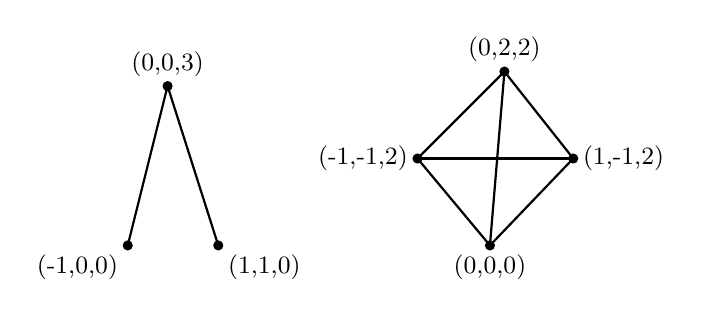
\begin{tikzpicture}[scale=0.92, every node/.style={font=\small}, line cap=round]
  \begin{scope}
    \coordinate (a0) at (0,0);
    \coordinate (a1) at (1.25,0);
    \coordinate (a2) at (0.55,2.2);
    \draw[thick] (a0) -- (a2) -- (a1);
    \foreach \p/\lab/\pos in {a0/{(-1,0,0)}/below left,a1/{(1,1,0)}/below right,a2/{(0,0,3)}/above}
      \fill (\p) circle (2pt) node[\pos] {\lab};
  \end{scope}

  \begin{scope}[xshift=5.0cm]
    \coordinate (b0) at (0,0);
    \coordinate (b1) at (-1.0,1.2);
    \coordinate (b2) at (1.15,1.2);
    \coordinate (b3) at (0.2,2.4);
    \draw[thick] (b0) -- (b1) -- (b3) -- (b2) -- (b0);
    \draw[thick] (b1) -- (b2);
    \draw[thick] (b0) -- (b3);
    \foreach \p/\lab/\pos in {b0/{(0,0,0)}/below,b1/{(-1,-1,2)}/left,b2/{(1,-1,2)}/right,b3/{(0,2,2)}/above}
      \fill (\p) circle (2pt) node[\pos] {\lab};
  \end{scope}
\end{tikzpicture}
\caption{Hai cấu trúc mẫu trong \textit{Ars Longa}: cấu trúc bên trái thiếu ràng buộc nên không tĩnh; cấu trúc bên phải có thêm thanh nối giữa các khớp treo, nhưng vẫn cần kiểm tra hạng của hệ tuyến tính để kết luận ổn định.}
\end{figure}

\subsection{Cân bằng và ổn định}

Do mô hình đã được tuyến tính hóa, cấu trúc cân bằng khi và chỉ khi hệ phương
trình có nghiệm. Ta dùng khử Gauss. Nếu sau khi khử xuất hiện hàng có mọi hệ
số bằng \(0\) nhưng vế phải khác \(0\), hệ vô nghiệm và cấu trúc không cân
bằng. Ngược lại, có nghiệm.

Ổn định thoạt nhìn phức tạp hơn: dù có tác dụng thêm lực tùy ý vào các điểm,
cấu trúc vẫn phải giữ được cân bằng. Trong ngôn ngữ phương trình, điều này
tương ứng với việc thay đổi vế phải rồi hỏi hệ có còn nghiệm hay không. Sau
khi khử Gauss, nếu tồn tại hàng hệ số toàn \(0\), thì chỉ cần thay đổi vế phải
của hàng ấy là hệ có thể vô nghiệm, nên cấu trúc không ổn định. Nếu không có
hàng hệ số toàn \(0\), mọi vế phải đều biểu diễn được, nên cấu trúc ổn định.

Như vậy bài toán vật lý được đưa về đại số tuyến tính. Với \(\Oh(N)\) phương
trình và \(\Oh(M)\) ẩn, chi phí khử Gauss ở quy mô \(N,M\le100\) là thoải mái.

\subsection{Về dữ liệu suy biến}

Bản gốc cũng thảo luận các trường hợp suy biến, chẳng hạn các thanh kề một
điểm cùng nằm trong một mặt phẳng gây ra diễn giải lực vô hạn không thực tế.
Những tình huống này cho thấy khi mô hình hóa vật lý, ta cần rất nghiêm ngặt
về giả thiết. Một đề tốt nên tránh hoặc định nghĩa rõ các dữ liệu suy biến;
nếu không, mô hình toán học có thể cho kết quả khác với trực giác vật lý.

\section{Water Tanks}

\subsection{Từ mô phỏng tới quy luật}

Bài \textit{Water Tanks} có \(N\) bình trụ đáy bằng nhau xếp thành hàng. Bình
đầu hở, các bình còn lại kín. Giữa các bình kề nhau có ống nối ngang ở các độ
cao cho trước. Nước và không khí đi qua ống; nước không nén được, không khí
nén được theo quy luật \(P_1V_1=P_2V_2\). Cần tính lượng nước đã đổ vào khi
bình đầu đầy.

\begin{figure}[htbp]
\centering
\begin{tikzpicture}[x=0.7cm,y=0.54cm, every node/.style={font=\small}]
  \newcommand{\tank}[4]{
    \draw (#1,0) rectangle ++(0.9,#2);
    \ifdim #3pt>0pt
      \fill[blue!28] (#1,0) rectangle ++(0.9,#3);
    \fi
    \draw (#1,#4) -- ++(0.9,0);
  }
  \begin{scope}
    \tank{0}{6.0}{0.0}{3.0}
    \tank{1.9}{4.8}{0.0}{3.0}
    \draw[thick] (0.9,3.0) -- (1.9,3.0);
    \node[below] at (1.35,-0.35) {trước khi đổ};
  \end{scope}
  \begin{scope}[xshift=5.2cm]
    \tank{0}{6.0}{6.0}{3.0}
    \tank{1.9}{4.8}{3.45}{3.0}
    \draw[thick] (0.9,3.0) -- (1.9,3.0);
    \node[below] at (1.35,-0.35) {sau khi bình 1 đầy};
    \node[right] at (2.9,4.15) {\(\,P>1\)};
  \end{scope}
\end{tikzpicture}
\caption{Trường hợp hai bình: khí trong bình kín bị nén, nên mực nước cuối cùng ở bình thứ hai thấp hơn mực nước ở bình hở.}
\end{figure}

Mô phỏng trực tiếp rất dễ rối: khi mặt nước qua một ống, các khoang không khí
có thể nối hoặc tách; áp suất của nhiều bình thay đổi phụ thuộc lẫn nhau. Vì
thế lời giải bắt đầu từ một số tính chất đơn giản:
\begin{itemize}
  \item nếu mặt nước ở bình \(i\) chưa tới ống nối sang \(i+1\), thì bình
  \(i+1\) chưa nhận nước từ bên trái;
  \item nếu mặt nước ở bình \(i+1\) chưa tới độ cao ống, hai khoang còn thông;
  nếu đã vượt, chúng tách nhau;
  \item khi một bình đã tách khỏi hai bên, thể tích khí còn lại và áp suất của
  nó chỉ phụ thuộc vào cột nước cao nhất, có thể xét riêng.
\end{itemize}

\subsection{Trường hợp độ cao ống tăng dần}

Với trường hợp đặc biệt độ cao các ống tăng từ trái sang phải, quá trình có
các giai đoạn rõ ràng. Nước làm bình kế tiếp dâng tới độ cao ống, rồi hai phần
khí bị tách, bình bên trái trở thành một phần đã có thể xử lý riêng. Mỗi giai
đoạn chỉ cần giải một phương trình một ẩn về độ tăng mặt nước, dựa trên áp suất
khí và áp suất cột nước.

Vì mỗi bình tham gia một số giai đoạn hằng số, trường hợp đặc biệt này giải
được trong \(\Oh(N)\).

\subsection{Từ đặc biệt tới tổng quát}

Với độ cao ống tùy ý, bản gốc nhóm các bình thành các \term{khối}. Một khối là
một đoạn bình liên tiếp mà các độ cao ống có quan hệ đơn điệu phù hợp; cả khối
đóng vai trò như một bình trong mô hình đặc biệt. Bên trong khối, khi cần xử
lý, ta đi ngược dần qua các ống để xác định bình nào dâng tới độ cao nào và
khi nào bị tách.

\begin{figure}[htbp]
\centering
\begin{tikzpicture}[x=0.52cm,y=0.43cm, every node/.style={font=\scriptsize}]
  \newcommand{\rowtanks}[3]{
    \begin{scope}[yshift=#1]
      \foreach \x/\h/\w in {0/7/#2,1.5/5.4/#3,3.0/6.2/0,4.5/4.6/0,6.0/7.4/0} {
        \draw (\x,0) rectangle ++(0.9,\h);
        \ifnum\w>0
          \fill[blue!25] (\x,0) rectangle ++(0.9,\w);
        \fi
      }
      \draw[thick] (0.9,2.0) -- (1.5,2.0);
      \draw[thick] (2.4,3.0) -- (3.0,3.0);
      \draw[thick] (3.9,4.2) -- (4.5,4.2);
      \draw[thick] (5.4,5.2) -- (6.0,5.2);
    \end{scope}
  }
  \rowtanks{0cm}{1}{0}
  \rowtanks{-3.1cm}{2}{2}
  \rowtanks{-6.2cm}{3}{3}
  \rowtanks{-9.3cm}{4}{4}
  \draw[-{Latex[length=2mm]}] (7.6,-0.4) -- (7.6,-2.5);
  \draw[-{Latex[length=2mm]}] (7.6,-3.5) -- (7.6,-5.6);
  \draw[-{Latex[length=2mm]}] (7.6,-6.6) -- (7.6,-8.7);
  \node[right] at (8.0,-1.5) {tách khối};
  \node[right] at (8.0,-4.6) {dâng tiếp};
  \node[right] at (8.0,-7.7) {gom đoạn đơn điệu};
\end{tikzpicture}
\caption{Ý tưởng nhóm bình thành các khối: thay vì theo dõi từng khoang khí toàn cục, thuật toán xử lý các đoạn có cùng kiểu chuyển tiếp rồi thu gọn chúng thành một đơn vị.}
\end{figure}

Điểm quan trọng là toàn bộ các thao tác trong một khối có chi phí tỉ lệ với
kích thước khối. Tổng kích thước các khối là \(N\), nên thuật toán tổng quát
vẫn giữ được \(\Oh(N)\) thời gian và \(\Oh(N)\) bộ nhớ.

Ví dụ này thể hiện một phương pháp thường gặp: trước hết hiểu một trường hợp
đặc biệt có trật tự, sau đó tìm cách gom dữ liệu tổng quát thành các đơn vị
ứng xử giống trường hợp đặc biệt.

\section{3D Musical Water-fence}

\subsection{Tính giao hoán của thao tác đổ nước}

Bài \textit{3D Musical Water-fence} có lưới \(N\times M\), mỗi ô có độ cao
khác nhau. Mỗi thao tác đổ một lượng nước vào một ô. Nước chảy từ cao xuống
thấp; khi tạo thành vùng nước cùng mực, nước dâng tới khi gặp lỗ thoát thấp
nhất rồi tràn đi. Cần tính tổng lượng nước lãng phí chảy ra ngoài lưới sau
\(T\) thao tác.

\begin{figure}[htbp]
\centering

\includegraphics[width=0.52\linewidth]{\assetbase/terrain-example.png}
\caption{Ví dụ địa hình \(4\times4\) trong \textit{3D Musical Water-fence}; các ô thấp ở giữa tạo thành bồn trũng giữ nước trước khi tràn qua cửa thấp nhất.}
\end{figure}

Mô phỏng đúng theo thứ tự thao tác có thể bùng nổ: một lượng nước đổ ở đỉnh
cao có thể chia nhánh qua rất nhiều ô. Trực giác đầu tiên của bản gốc là thử
hỏi: nếu đổi thứ tự hai thao tác đổ nước, kết quả cuối có thay đổi không?
Phân tích cho thấy không. Khi nước từ thao tác sau đáng lẽ đi vào một ô đã
được nâng mực bởi thao tác trước, lượng nước dư cuối cùng vẫn tràn ra theo
cùng đường thoát. Do đó các thao tác đổ nước có thể gom lại và xử lý theo thứ
tự thuận tiện.

Từ đây, ta có thể cộng tổng lượng nước đổ vào từng ô, rồi xử lý các ô theo độ
cao giảm dần. Cách này loại bỏ đệ quy chảy nước của từng thao tác riêng lẻ.

\subsection{Nén bồn trũng}

Mô phỏng vùng nước dâng vẫn có thể đắt nếu mỗi lần đều BFS vùng cùng mực. Bản
gốc tiếp tục nén thông tin bằng khái niệm \term{bồn trũng}. Mỗi ô có một mực
nước cuối cùng nếu đổ vô hạn nước vào toàn lưới. Một bồn trũng ở cao độ \(h\)
là một vùng liên thông các ô có mực cuối cùng bằng \(h\), độ cao gốc nhỏ hơn
\(h\), và chỉ tràn qua một ô cửa ở cao độ \(h\). Dung tích của bồn là
\[
  h\cdot |B|-\sum_{u\in B}height(u).
\]

Nếu tổng nước rơi vào bồn không vượt quá dung tích, không có gì tràn ra. Nếu
vượt, chỉ lượng dư cần đẩy qua cửa tràn. Ta không cần mô phỏng mực nước chi
tiết trong bồn.

Thuật toán:
\begin{enumerate}
  \item duyệt ô theo độ cao tăng dần để xác định cửa tràn và các bồn trũng,
  đồng thời tính dung tích;
  \item thống kê tổng lượng nước ban đầu tại mỗi ô/cửa/bồn;
  \item xử lý các cửa theo cao độ giảm dần: đẩy nước xuống bồn thấp hơn, cửa
  thấp hơn, hoặc ra ngoài lưới; nếu bồn quá dung tích thì chỉ đẩy lượng dư qua
  cửa của nó;
  \item cộng lượng nước chảy ra ngoài làm đáp án.
\end{enumerate}

Mỗi ô được đưa vào một bồn hoặc là cửa tràn; mỗi quan hệ lân cận được xét một
số lần hằng số. Do đó tổng thời gian và bộ nhớ là \(\Oh(NM)\), đủ cho lưới rất
lớn.

\section{Kết luận}

Các bài toán có hương vị vật lý thường có hai mặt. Chúng rất trực quan, vì mô
tả một quá trình thật; nhưng cũng dễ đánh lừa, vì mô phỏng trực tiếp quá nhiều
chi tiết sẽ sinh ra vô số trường hợp. Cách tiếp cận hiệu quả là:
\begin{itemize}
  \item dùng trực giác vật lý để nhận ra đại lượng bảo toàn hoặc quy luật dòng
  chảy, cân bằng, ổn định;
  \item chuyển quy luật ấy thành phương trình, phân đoạn, khối, bồn trũng hoặc
  cấu trúc dữ liệu;
  \item chứng minh các bước nén/thay đổi thứ tự không làm đổi kết quả.
\end{itemize}

Những lời giải sau khi tìm ra thường không quá dài, nhưng quá trình đi tới
chúng đòi hỏi kiên nhẫn, tưởng tượng không gian và phân tích nghiêm ngặt. Đây
cũng là lý do lớp bài này ngày càng phù hợp với xu hướng đề thi tin học hiện
đại.

\section*{Ghi chú về nguồn}

Tệp gốc có mục lục Word cũ, nhiều hình và ba phát biểu bài liên quan. Các hình
chính dùng trong lập luận đã được phục dựng thành TikZ hoặc giữ bằng ảnh địa
hình nhỏ, không còn chú thích treo không kèm hình. Ba tệp bài riêng
\textit{3D Musical Water-fence}, \textit{Water Tanks} và \textit{Ars Longa}
có bản dịch riêng trong cùng thư mục; bản dịch này tập trung vào bài luận
phương pháp tổng quát của Fang Ge và chỉ tóm lược phát biểu đề khi cần cho
phân tích.

\end{document}
